\documentclass[aspectratio=169,10pt]{beamer}
\usepackage[utf8]{inputenc}
\usepackage[T1]{fontenc}
\usepackage{amsmath,amsfonts,amssymb}
\usepackage{graphicx}
\usepackage{xcolor}
\usepackage{tikz}
\usetikzlibrary{shapes,arrows.meta,positioning,fit,calc,shadows}
\usepackage{booktabs}
\usepackage{array}
\usepackage{colortbl}
\usepackage{listings}
\usepackage{hyperref}

\usetheme{Madrid}
\usecolortheme{default}
\setbeamertemplate{navigation symbols}{}
\setbeamertemplate{footline}[frame number]

\AtBeginSection[]{}
\AtBeginSubsection[]{}

\definecolor{mlblue}{RGB}{0,102,204}
\definecolor{mlgreen}{RGB}{0,153,76}
\definecolor{mlorange}{RGB}{255,102,0}
\definecolor{mlred}{RGB}{204,0,51}
\definecolor{mlpurple}{RGB}{102,51,153}
\definecolor{codebg}{RGB}{245,245,248}

\setbeamercolor{structure}{fg=mlblue}
\setbeamercolor{block title}{bg=mlblue,fg=white}
\setbeamercolor{block body}{bg=mlblue!8}
\setbeamercolor{alerted text}{fg=mlred}
\setbeamercolor{example text}{fg=mlgreen}

\lstdefinestyle{pythonstyle}{
    language=Python,
    basicstyle=\ttfamily\scriptsize,
    keywordstyle=\color{mlblue}\bfseries,
    commentstyle=\color{mlgreen!70!black}\itshape,
    stringstyle=\color{mlred},
    showstringspaces=false,
    breaklines=true,
    frame=single,
    rulecolor=\color{gray!40},
    backgroundcolor=\color{codebg},
    numbers=left,
    numberstyle=\tiny\color{gray},
    numbersep=4pt,
    xleftmargin=1.2em
}
\lstset{style=pythonstyle}

\title[FastAPI]{From Model to Medium}
\subtitle{Topic 3: FastAPI (Python Web Framework)}
\author{ML + UI + API + MCP Project}
\institute{Learning Path}
\date{\today}

\begin{document}

\begin{frame}
\titlepage
\end{frame}

\begin{frame}{Outline}
\tableofcontents
\end{frame}

\section{What is FastAPI?}

\begin{frame}{Why FastAPI for our ML project?}
\begin{columns}[T]
\begin{column}{0.5\textwidth}
\begin{block}{Key idea}
FastAPI turns ordinary Python functions into web endpoints, and builds validation and documentation from the type hints.
\end{block}
\begin{itemize}
\item \textbf{Fast to write}: a few lines per endpoint.
\item \textbf{Automatic validation}: wrong types return \texttt{422}.
\item \textbf{Free docs}: Swagger UI at \texttt{/docs}.
\item \textbf{Python-native}: works with scikit-learn, pandas, joblib.
\end{itemize}
\end{column}
\begin{column}{0.46\textwidth}
\begin{alertblock}{ML application}
Our trained model becomes one function: \texttt{POST /v1/predictions} receives stats and returns the predicted power.
\end{alertblock}
\end{column}
\end{columns}
\end{frame}

\begin{frame}{The stack under the hood}
\begin{center}
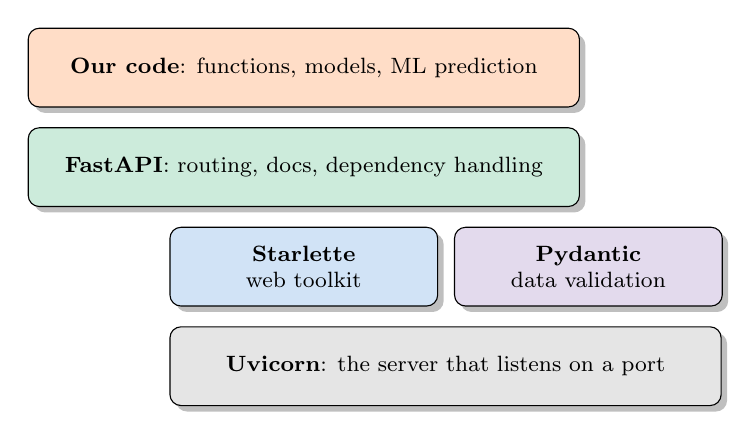
\begin{tikzpicture}[
  box/.style={draw, rounded corners, align=center, minimum height=1cm,
              minimum width=7cm, font=\footnotesize, drop shadow},
]
  \node[box, fill=mlorange!22] (code) {\textbf{Our code}: functions, models, ML prediction};
  \node[box, fill=mlgreen!20, below=0.25cm of code] (fast) {\textbf{FastAPI}: routing, docs, dependency handling};
  \node[box, fill=mlblue!18, below=0.25cm of fast, minimum width=3.4cm] (star) {\textbf{Starlette}\\web toolkit};
  \node[box, fill=mlpurple!18, right=0.2cm of star, minimum width=3.4cm] (pyd) {\textbf{Pydantic}\\data validation};
  \node[box, fill=gray!20, below=0.25cm of star, minimum width=7cm, xshift=1.8cm] (uvi) {\textbf{Uvicorn}: the server that listens on a port};
\end{tikzpicture}
\end{center}
\end{frame}

\section{Our first endpoints}

\begin{frame}[fragile]{Hello World}
\begin{columns}[T]
\begin{column}{0.55\textwidth}
\begin{lstlisting}
from fastapi import FastAPI

app = FastAPI(title="Hello API")


@app.get("/")
def hello():
    return {"message": "Hello, player one!"}
\end{lstlisting}
\end{column}
\begin{column}{0.4\textwidth}
\begin{enumerate}
\item \texttt{FastAPI()} creates the app.
\item The \textbf{decorator} links method + URL to the function.
\item A returned \texttt{dict} becomes \textbf{JSON}.
\end{enumerate}
\begin{exampleblock}{Response}
\texttt{200 OK}\\
\texttt{\{"message": "Hello, player one!"\}}
\end{exampleblock}
\end{column}
\end{columns}
\end{frame}

\begin{frame}{From request to function}
\begin{center}
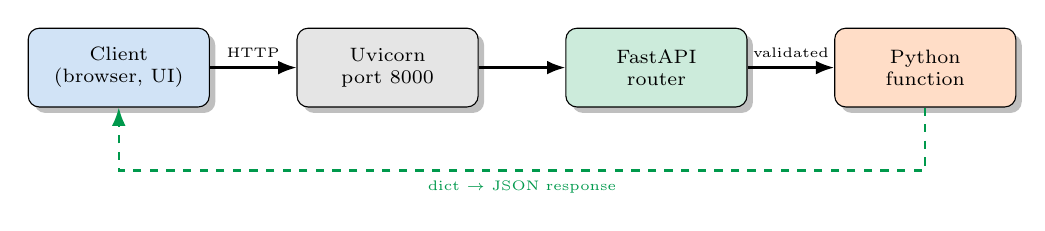
\begin{tikzpicture}[
  box/.style={draw, rounded corners, align=center, minimum height=1cm,
              minimum width=2.3cm, font=\scriptsize, drop shadow},
  arr/.style={-{Latex}, thick}
]
  \node[box, fill=mlblue!18] (c) {Client\\(browser, UI)};
  \node[box, fill=gray!20, right=1.1cm of c] (u) {Uvicorn\\port 8000};
  \node[box, fill=mlgreen!20, right=1.1cm of u] (f) {FastAPI\\router};
  \node[box, fill=mlorange!22, right=1.1cm of f] (fn) {Python\\function};
  \draw[arr] (c) -- node[above, font=\tiny] {HTTP} (u);
  \draw[arr] (u) -- (f);
  \draw[arr] (f) -- node[above, font=\tiny] {validated} (fn);
  \draw[arr, dashed, mlgreen] (fn.south) -- ++(0,-0.8) -| node[below, pos=0.25, font=\tiny] {dict $\rightarrow$ JSON response} (c.south);
\end{tikzpicture}
\end{center}
\end{frame}

\begin{frame}[fragile]{Path and query parameters}
\begin{lstlisting}
@app.get("/characters/{character_id}")           # path parameter
def one_character(character_id: int, verbose: bool = False):   # query parameter
    data = {"id": character_id, "name": "pikachu"}
    if verbose:
        data["stats"] = {"attack": 55, "defense": 40, "speed": 90}
    return data
\end{lstlisting}
\vspace{0.1cm}
\begin{center}
\begin{tabular}{lll}
\toprule
\textbf{Request} & \textbf{Result} & \textbf{Why} \\
\midrule
\texttt{/characters/25} & 200, basic data & \texttt{verbose} defaults to \texttt{False} \\
\texttt{/characters/25?verbose=true} & 200, with stats & query parameter read \\
\texttt{/characters/abc} & \alert{422} & \texttt{abc} is not an \texttt{int} \\
\bottomrule
\end{tabular}
\end{center}
\end{frame}

\section{The Game Power API}

\begin{frame}{Topic 2 contract $\rightarrow$ code}
\begin{center}
\begin{tabular}{lll}
\toprule
\textbf{Route} & \textbf{Function} & \textbf{Success / error} \\
\midrule
\texttt{GET /v1/characters} & \texttt{list\_characters} & 200, paginated \\
\texttt{GET /v1/characters/\{id\}} & \texttt{get\_character} & 200 / 404 \\
\texttt{POST /v1/predictions} & \texttt{create\_prediction} & 200 / 422 \\
\bottomrule
\end{tabular}
\end{center}
\vspace{0.2cm}
\begin{center}
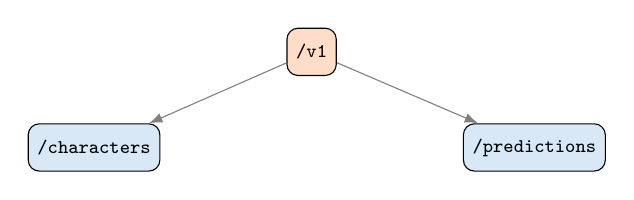
\begin{tikzpicture}[
  res/.style={draw, rounded corners, fill=mlblue!15, font=\scriptsize\ttfamily, minimum height=0.6cm, align=center},
  arr/.style={-{Latex}, gray}
]
  \node[res, fill=mlorange!22] (root) {/v1};
  \node[res, below left=0.6cm and 1.6cm of root] (ch) {/characters};
  \node[res, below right=0.6cm and 1.6cm of root] (pr) {/predictions};
  \draw[arr] (root) -- (ch);
  \draw[arr] (root) -- (pr);
\end{tikzpicture}
\end{center}
\end{frame}

\begin{frame}[fragile]{Pagination and 404 in FastAPI}
\begin{lstlisting}
@app.get("/v1/characters")
def list_characters(page: int = Query(1, ge=1), limit: int = Query(5, ge=1, le=50)):
    items = list(CHARACTERS.values())
    start = (page - 1) * limit
    return {"items": items[start:start + limit],
            "page": page, "limit": limit, "total": len(items)}


@app.get("/v1/characters/{character_id}")
def get_character(character_id: int):
    if character_id not in CHARACTERS:
        raise HTTPException(
            status_code=404,
            detail={"code": "CHARACTER_NOT_FOUND",
                    "message": f"Character {character_id} does not exist"})
    return CHARACTERS[character_id]
\end{lstlisting}
\end{frame}

\begin{frame}[fragile]{The prediction endpoint}
\begin{columns}[T]
\begin{column}{0.58\textwidth}
\begin{lstlisting}
from pydantic import BaseModel

class PredictionRequest(BaseModel):
    attack: int
    defense: int
    speed: int

class PredictionResponse(BaseModel):
    predicted_power: float
    model_version: str

@app.post("/v1/predictions",
          response_model=PredictionResponse)
def create_prediction(request: PredictionRequest):
    power = (1.5 * request.attack + request.defense
             + 0.5 * request.speed)
    return {"predicted_power": power,
            "model_version": "0.1.0"}
\end{lstlisting}
\end{column}
\begin{column}{0.38\textwidth}
\begin{alertblock}{Today vs.\ Topic 5}
The formula is a placeholder. Later the body becomes \texttt{model.predict(...)} with our trained regression.
\end{alertblock}
\begin{block}{Body type}
The function parameter typed as a Pydantic class tells FastAPI to read and validate the \textbf{JSON body}.
\end{block}
\end{column}
\end{columns}
\end{frame}

\section{Docs, Running, Testing}

\begin{frame}{Automatic documentation}
\begin{center}
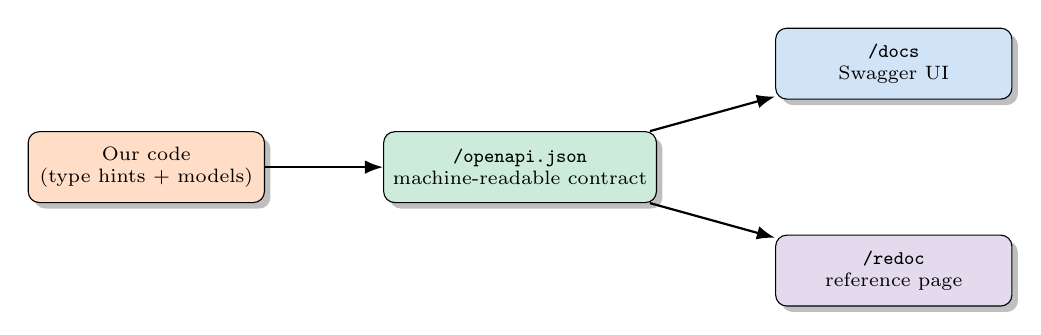
\begin{tikzpicture}[
  box/.style={draw, rounded corners, align=center, minimum height=0.9cm,
              minimum width=3cm, font=\scriptsize, drop shadow},
  arr/.style={-{Latex}, thick}
]
  \node[box, fill=mlorange!22] (code) {Our code\\(type hints + models)};
  \node[box, fill=mlgreen!20, right=1.5cm of code] (spec) {\texttt{/openapi.json}\\machine-readable contract};
  \node[box, fill=mlblue!18, above right=0.4cm and 1.5cm of spec] (docs) {\texttt{/docs}\\Swagger UI};
  \node[box, fill=mlpurple!18, below right=0.4cm and 1.5cm of spec] (redoc) {\texttt{/redoc}\\reference page};
  \draw[arr] (code) -- (spec);
  \draw[arr] (spec) -- (docs);
  \draw[arr] (spec) -- (redoc);
\end{tikzpicture}
\end{center}
\begin{block}{Remember}
Change the code and the docs update themselves: documentation can never be out of date.
\end{block}
\end{frame}

\begin{frame}[fragile]{Running the server}
\begin{lstlisting}[language=bash, numbers=none]
# in the folder that contains 03_game_api.py
uvicorn 03_game_api:app --reload --port 8000
\end{lstlisting}
\begin{center}
\begin{tabular}{lll}
\toprule
\textbf{Part} & \textbf{Meaning} & \textbf{Tip} \\
\midrule
\texttt{03\_game\_api} & Python file (no \texttt{.py}) & run from that folder \\
\texttt{app} & variable inside the file & name must match \\
\texttt{--reload} & restart on every save & development only \\
\texttt{--port 8000} & where to listen & change if busy \\
\bottomrule
\end{tabular}
\end{center}
Then open \texttt{http://127.0.0.1:8000/docs} and use \textbf{Try it out}.
\end{frame}

\begin{frame}[fragile]{Testing without a server: TestClient}
\begin{lstlisting}
from fastapi.testclient import TestClient
from game_api import app

client = TestClient(app)

def test_prediction():
    r = client.post("/v1/predictions",
                    json={"attack": 55, "defense": 40, "speed": 90})
    assert r.status_code == 200
    assert r.json()["predicted_power"] == 167.5

def test_missing_character():
    assert client.get("/v1/characters/99").status_code == 404
\end{lstlisting}
\end{frame}

\begin{frame}{Status codes we get for free}
\begin{center}
\begin{tabular}{lll}
\toprule
\textbf{Situation} & \textbf{Code} & \textbf{Who decides} \\
\midrule
\rowcolor{mlgreen!12} Valid request & 200 & our function returns \\
\rowcolor{mlorange!15} Character not found & 404 & we raise \texttt{HTTPException} \\
\rowcolor{mlred!12} Text instead of a number & 422 & FastAPI + Pydantic \\
\rowcolor{mlred!12} GET on a POST route & 405 & FastAPI \\
\rowcolor{mlorange!15} Unknown URL & 404 & FastAPI \\
\bottomrule
\end{tabular}
\end{center}
\end{frame}

\section{Takeaways}

\begin{frame}{Takeaways}
\begin{enumerate}
\item \textbf{Decorator + function} = endpoint; the return value becomes JSON.
\item \textbf{Type hints} validate path, query and body data automatically.
\item \textbf{Pydantic models} describe the JSON body and the response shape.
\item \textbf{Uvicorn} runs the server; \texttt{--reload} helps while learning.
\item \textbf{/docs} and \textbf{TestClient} let us try and test without extra tools.
\item Next topic: \textbf{Data Validation with Pydantic}.
\end{enumerate}
\end{frame}

\end{document}
